\vspace{-1.5em}

Um die angekreuzte Antwort auf eine Frage herauszufinden, müssen Sie innerhalb des Vierecks nach den entsprechenden Kästchen suchen.
\begin{itemize}
\item Für jede der Antwortmöglichkeiten von + + bis - - schneiden Sie das zugehörige Kästchen großzügig als eigenes Bild heraus.
\item Für spätere Verarbeitung ist es wichtig sicherzustellen, dass diese Ausschnitte zu den vorhandenen Daten passen.
Betrachten Sie dazu Beispiele aus der Sammlung \lstinline{crosses.tar.gz}.
\item Skalieren Sie das ausgeschnittene Bild des Kästchens auf eine fixe Größe von 40x40 Pixel.
\end{itemize}
Leeres und angekreuztes Kästchen (zur Verdeutlichung mit Rahmen)\\
\begin{center}
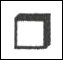
\includegraphics{bilder/cross_empty_example.png}
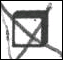
\includegraphics{bilder/cross_crossed_example.png}\\
\end{center}

Doch wie finden wir nun heraus, was es bedeutet \emph{angekreuzt} zu sein? Die Kreuze sind kreuz und quer und mit sehr verschiedenen Stiften gemalt...
\vspace{1.5em}
